\subsection{Character, trace identities, and the abelian index}

\begin{proposition}[Split weight enumerator and one-family character]
\label{prop:split-weight-enumerator}
For the present paragraph let
\[
\chi_{S^+}(t):=\tr_{S^+}(e^{tY}).
\]
Define also the split weight enumerator
\[
W(u,v)
:=
\sum_{\substack{0\le n_3\le 3\\ 0\le n_2\le 2\\ n_3+n_2\ \mathrm{even}}}
\binom{3}{n_3}\binom{2}{n_2}u^{n_3}v^{n_2}.
\]
Then
\begin{equation}
\label{eq:split-weight-enumerator}
W(u,v)
=
1+3u^2+6uv+v^2+2u^3v+3u^2v^2
=
\frac12\Big[(1+u)^3(1+v)^2+(1-u)^3(1-v)^2\Big].
\end{equation}
Moreover,
\begin{equation}
\label{eq:family-character}
\chi_{S^+}(t)
=
\frac12\Big[
\bigl(1+e^{-t/3}\bigr)^3\bigl(1+e^{t/2}\bigr)^2
+
\bigl(1-e^{-t/3}\bigr)^3\bigl(1-e^{t/2}\bigr)^2
\Big]
=
W(e^{-t/3},e^{t/2}).
\end{equation}
Consequently,
\[
\chi_{S^+}(0)=16,
\qquad
\chi_{S^+}'(0)=\tr_{S^+}Y=0,
\qquad
\chi_{S^+}''(0)=\tr_{S^+}Y^2=\frac{10}{3},
\qquad
\chi_{S^+}'''(0)=\tr_{S^+}Y^3=0.
\]
\end{proposition}

\begin{remark}[Master generating function for the one-family packet]
The even-parity split weight enumerator
\[
W(u,v)=\frac12\bigl[(1+u)^3(1+v)^2+(1-u)^3(1-v)^2\bigr]
\]
is the master generator of the family packet. The one-family character is obtained by the
specialization $u=e^{-t/3}$ and $v=e^{t/2}$, while all trace moments of $Y$ are recovered by
differentiating at $t=0$.
\end{remark}

\begin{proof}
The pairs $(n_3,n_2)$ allowed by even total degree are
\[
(0,0),\ (2,0),\ (1,1),\ (0,2),\ (3,1),\ (2,2),
\]
with multiplicities
\[
1,\ 3,\ 6,\ 1,\ 2,\ 3.
\]
This gives the explicit polynomial formula for $W(u,v)$. Equivalently, the parity projector
\[
\frac12\bigl(1+(-1)^{n_3+n_2}\bigr)
\]
acting on $(1+u)^3(1+v)^2$ yields \Cref{eq:split-weight-enumerator}. Substituting
\[
u=e^{-t/3},
\qquad
v=e^{t/2}
\]
gives \Cref{eq:family-character}. For an even exterior algebra one also has
\[
\tr_{\Lambda^{\mathrm{even}}E}(e^{tY})
=
\frac12\Big[\prod_{j=1}^5(1+e^{tq_j})+\prod_{j=1}^5(1-e^{tq_j})\Big],
\]
with carrier charges $q_j\in\{-1/3,-1/3,-1/3,1/2,1/2\}$. Differentiating at $t=0$ yields the stated dimension and trace identities.
\end{proof}

\begin{corollary}[Multiplicative character as six-sector decoder]
\label{cor:multiplicative-family-character}
Let
\[
X:=6Y.
\]
Then the multiplicative one-family character
\[
\Xi_{S^+}(t):=\tr_{S^+}(t^X)
\]
is
\begin{equation}
\label{eq:multiplicative-family-character}
\Xi_{S^+}(t)
=
\frac12\Big[
(1+t^{-2})^3(1+t^3)^2
+
(1-t^{-2})^3(1-t^3)^2
\Big]
=
t^6+3t^2+6t+1+2t^{-3}+3t^{-4}.
\end{equation}
Consequently
\[
\Xi_{S^+}(1)=16,
\qquad
(t\partial_t)\Xi_{S^+}(1)=\tr_{S^+}X=0,
\qquad
(t\partial_t)^2\Xi_{S^+}(1)=\tr_{S^+}X^2=120=5!.
\]
Thus the six sectors and their multiplicities are read off directly from the monomials of
\Cref{eq:multiplicative-family-character}.
\end{corollary}

\begin{proof}
Since $X=3N_2-2N_3$, every admissible occupancy pair contributes the monomial
$t^{3n_2-2n_3}$. Therefore
\[
\Xi_{S^+}(t)=W(t^{-2},t^3),
\]
and \Cref{eq:split-weight-enumerator} gives the displayed factorized form. Expanding yields the six
monomials shown above. Applying $t\partial_t$ once and twice at $t=1$ recovers the first two trace
moments of $X$.
\end{proof}

\begin{remark}[Table as readout, character as proof device]
The one-family table remains useful as a reader-facing decoding sheet, but the whole six-sector
arithmetic is already compressed into the single multiplicative character
\Cref{eq:multiplicative-family-character}.
\end{remark}

\begin{remark}[Six admissible occupancy sectors]
The six monomials in \Cref{eq:split-weight-enumerator} are exactly the six allowed occupancy pairs $(n_3,n_2)$ of the family packet. This is the shortest combinatorial route from the split carrier to the six Standard Model multiplet sectors listed in \Cref{tab:one-family}.
\end{remark}

The carrier packet therefore reproduces the standard trace cancellations
\[
\tr_{S^+}Y=0,
\qquad
\tr_{S^+}Y^3=0,
\]
and packages them together with the quadratic trace in one formula. Since $\tr_{S^+}Y^2=4\gamma=10/3$ and $\tr_\Phi Y^2=1/2$ for one weak doublet with hypercharge $1/2$, the hypercharge trace coefficient organizes as
\begin{equation}
\label{eq:abelian-index}
\bone(N_{\mathrm{fam}},N_\Phi)
=
\frac25N_{\mathrm{fam}}\tr_{S^+}Y^2+\frac15N_\Phi\tr_\Phi Y^2
=
\frac85N_{\mathrm{fam}}\gamma+\frac1{10}N_\Phi
=
\frac43N_{\mathrm{fam}}+\frac1{10}N_\Phi.
\end{equation}
On the canonical branch $(N_{\mathrm{fam}},N_\Phi)=(3,1)$ this gives
\[
\bone=\frac{41}{10}.
\]
The abelian index is therefore not inserted as an isolated Standard Model datum; it is a carrier-level output once the family and Higgs counts are declared.

\begin{remark}[Canonical-branch Diophantine lock]
If one imposes $\bone=41/10$ on nonnegative integer data, then
\[
40N_{\mathrm{fam}}+3N_\Phi=123.
\]
The physically nontrivial solution is $(N_{\mathrm{fam}},N_\Phi)=(3,1)$, so the canonical branch is already sharply constrained at the level of the trace arithmetic.
\end{remark}

\begin{proposition}[Family hypercharge arithmetic and compression]
\label{prop:family-hypercharge-compression}
Let $N_3$ and $N_2$ be the occupation-number operators on the $E_3$ and $E_2$ slots, restricted to $S^+$, and define the scaled hypercharge operator
\[
X:=6Y=3N_2-2N_3.
\]
Then on $S^+$ one has
\begin{align}
X&\equiv N_2\equiv N_3 \pmod 2,\label{eq:x-mod-2}\\
X&\equiv N_3 \pmod 3,\label{eq:x-mod-3}\\
X&\equiv 3(N_2+N_3) \pmod 5.\label{eq:x-mod-5}
\end{align}
In particular, the even exterior degree $k=N_2+N_3\in\{0,2,4\}$ is read off from the residue class of $X$ modulo $5$: if $X\equiv r\pmod 5$ with $r\in\{0,1,2\}$, then $k=2r$, so
\[
X\bmod 5=0,1,2
\qquad\Longleftrightarrow\qquad
\Lambda^0E,\ \Lambda^2E,\ \Lambda^4E.
\]
Moreover,
\[
\mathrm{Spec}(X|_{S^+})=\{0,-4,1,6,-3,2\},
\]
and therefore
\begin{equation}
\label{eq:family-x-polynomial}
X(X+4)(X-1)(X-6)(X+3)(X-2)=0
\qquad\text{on }S^+.
\end{equation}
\end{proposition}

\begin{proof}
Each occupied $E_3$ mode contributes hypercharge $-1/3$ and each occupied $E_2$ mode contributes $+1/2$, so multiplying by $6$ gives $X=3N_2-2N_3$. Modulo $2$, the term $-2N_3$ vanishes, so $X\equiv N_2$. Because $S^+$ has even total degree, $N_2\equiv N_3\pmod 2$, which proves \Cref{eq:x-mod-2}. Modulo $3$, one has $3N_2\equiv 0$ and $-2\equiv 1$, giving \Cref{eq:x-mod-3}. Modulo $5$, the congruence $-2\equiv 3$ yields \Cref{eq:x-mod-5}. Since on $S^+$ the even degree is $k=N_2+N_3\in\{0,2,4\}$, the possible residues are $3k\equiv 0,1,2\pmod 5$, from which $k=2r$ with $r=X\bmod 5$ follows. Evaluating $X=3n_2-2n_3$ on the six admissible occupancy pairs $(n_3,n_2)$ gives the listed spectrum. The polynomial \Cref{eq:family-x-polynomial} is then the spectral polynomial with these six simple roots.
\end{proof}

\begin{corollary}[Five-fold phase filters for even degree]
\label{cor:family-degree-filters}
Let
\[
\zeta_5=e^{2\pi i/5},
\qquad
U_5:=e^{2\pi iX/5}.
\]
Then the even-degree projectors are the discrete Fourier filters
\[
P_{\Lambda^{2m}E}
=
\frac15\sum_{r=0}^{4}\zeta_5^{-mr}U_5^r,
\qquad
m=0,1,2.
\]
\end{corollary}

\begin{proof}
By \Cref{prop:family-hypercharge-compression}, the eigenspaces $\Lambda^{2m}E$ carry the residue class $X\equiv m\pmod 5$. Hence $U_5$ has eigenvalue $\zeta_5^m$ on $\Lambda^{2m}E$, and the standard Fourier projector formula on the cyclic group $\mathbb Z_5$ gives the claim.
\end{proof}

\begin{remark}[From the two-point carrier to the six-point family algebra]
The minimal carrier itself is a two-point algebra, but the family packet lifts the scaled hypercharge to a six-point algebra. Therefore every analytic function of $X$ on $S^+$ reduces to a polynomial of degree at most five. If
\[
M_n:=\tr_{S^+}(X^n),
\]
then \Cref{eq:family-x-polynomial} implies the finite recursion
\[
M_{n+6}
=
2M_{n+5}+31M_{n+4}-20M_{n+3}-156M_{n+2}+144M_{n+1}.
\]
In this sense the whole hypercharge statistics of one family is finitely compressed into six spectral values.
\end{remark}

\section{Kernel numerics and electromagnetic closure}

The boundary-to-carrier presentation should not leave the impression that TFPT is hard only at the level of group theory and representation bookkeeping. The numerical kernel already fixes a nontrivial output layer. Here that layer is pulled forward and read as the first established output package of the carrier/output architecture rather than as a later list of disconnected constants.

\begin{theorem}[Primitive seam generator]
\label{thm:primitive-seam-generator}
The primitive relative seam loop defines the positive generator
\[
[u_\Sigma]=1\in K^1(S^1)\cong \mathbb Z.
\]
Hence the associated seam spectral flow is
\[
SF(U_\Seam)=1,
\qquad
\Delta_\Seam=2\pi.
\]
In the relative Chern normalization, the seam constant is
\[
\cthree:=\frac{\Delta_\Seam}{16\pi^2}=\frac{1}{8\pi}.
\]
Moreover the seam-even base opening is the normalized complement of the carrier quadratic norm,
\[
\phibase
:=
\frac{1-\gamma}{\pi}
=
\frac{1-\tr_EY^2}{\pi}
=
\frac{1}{6\pi}.
\]
\end{theorem}

\begin{proof}[Proof sketch]
The primitive reconstruction yields one elementary relative seam class and therefore one primitive
generator of the seam $K^1$ lattice. Along a single positive seam circuit the spectral flow changes
by one, so the associated loop has class $[u_\Sigma]=1$ and spectral flow $SF(U_\Seam)=1$. The
primitive circuit closes after one full turn, giving $\Delta_\Seam=2\pi$ and hence
$\cthree=\Delta_\Seam/(16\pi^2)=1/(8\pi)$. The carrier theorem gives
$\gamma=\tr_EY^2=5/6$, so the seam-even opening is the normalized complement of the carrier
quadratic norm rather than a new independent numerical input.
\end{proof}

\begin{remark}[Interpretive picture of the primitive start state]
At the level of physical intuition, the primitive spectral seed may be read as a minimal nontrivial relative defect state: two sheets, one seam, one elementary relative winding, and an undecomposed internal rank-$5$ kernel before the carrier split is imposed. This is only an interpretive picture, not a new theorem. Its role is to explain why the earliest hard numbers $(\cthree,\phibase)$ already look like seam-normalized responses of a genuinely relative starting configuration.
\end{remark}

\begin{figure}[t]
\centering
\scriptsize
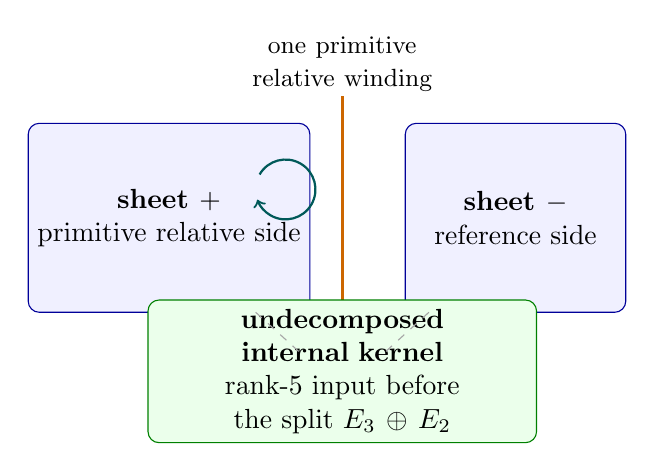
\begin{tikzpicture}[
    sheet/.style={draw=blue!60!black, fill=blue!6, rounded corners, minimum width=2.8cm, minimum height=2.4cm, align=center},
    kernel/.style={draw=green!50!black, fill=green!8, rounded corners, text width=4.7cm, minimum height=0.95cm, align=center}
]
\node[sheet] (up) at (-2.2,0) {\textbf{sheet $+$}\\primitive relative side};
\node[sheet] (down) at (2.2,0) {\textbf{sheet $-$}\\reference side};
\draw[orange!80!black, line width=1.2pt] (0,-1.55) -- (0,1.55);
\node[orange!80!black, above] at (0,1.55) {$\Seam$};
\draw[->, thick, teal!70!black] (-1.05,0.55) arc[start angle=150,end angle=-160,radius=0.38];
\node[align=center, text width=3.0cm] at (0,1.95) {\small one primitive\\relative winding};
\node[kernel] (k) at (0,-1.95) {\textbf{undecomposed internal kernel}\\rank-$5$ input before the split $E_3\oplus E_2$};
\draw[dashed, gray!70] (-1.1,-1.2) -- (-0.55,-1.7);
\draw[dashed, gray!70] (1.1,-1.2) -- (0.55,-1.7);
\end{tikzpicture}
\caption{Interpretive primitive start sketch. Two sheets, one seam, one elementary relative winding,
and an undecomposed rank-$5$ kernel appear before the later split into $E_3\oplus E_2$.
The picture is heuristic only; the theorem-level data are reconstructed from the one-sided
boundary datum.}
\label{fig:primitive-start-sketch}
\end{figure}

